\begin{figure}[t]
\begin{centering}
    % \subfloat[this will show up directly below the image]
                            % trim=left bottom right top, clip
    {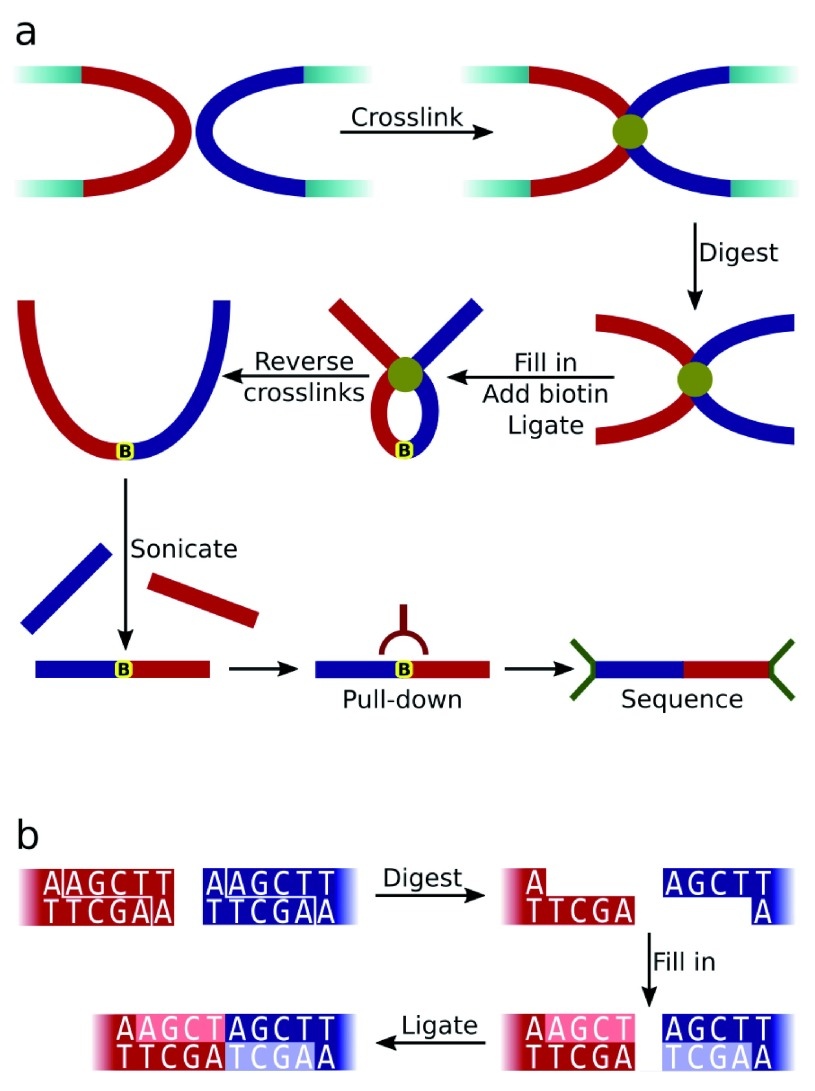
\includegraphics[scale=4,trim=0 40 0 6, clip]{figures/background/f1000research-4-7903-g0000.jpg}}
    \caption[Summarised Hi-C protocol]
    {\textbf{Summarised Hi-C protocol.}
    Biotin is shown by a yellow marker, while the red and blue parts are
    different parts of cross-linked fragments.
    The steps are explained in detail in \secref{sec:common} and \secref{sec:HiC}.
    \\ \\ Image taken from \cite{wingett2015hicup}.}
    \label{fig:HiC}
\end{centering}
\end{figure}

